\section{Accepttest}
Der kan ses ud fra målingerne at frekvensgangen ved 2 V, afbilledet på figur \ref{fig:acceff:frek2v}, ved de lave frekvenser, ikke er tilfredsstillende. Da frekvensgangen for 2 V og 200 mV bedømmes til at være meget ens, konkluderes der kun på frekvensgangen for 2 V.

\begin{figure}[h]
\centering
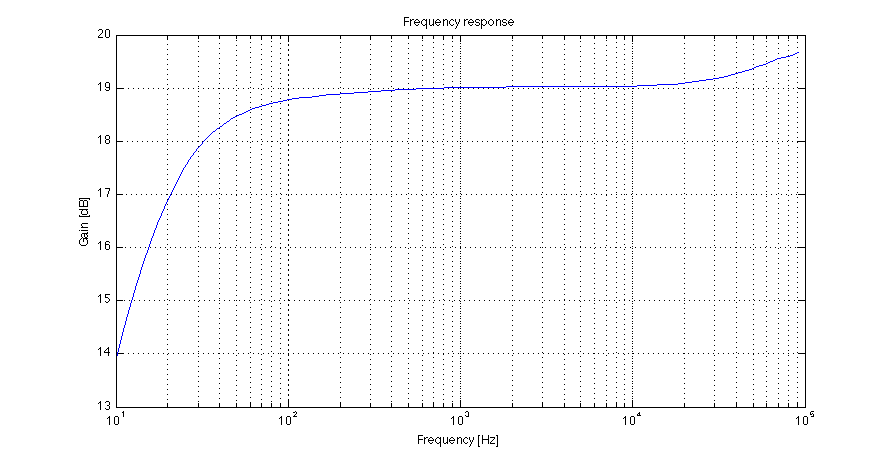
\includegraphics[width=\textwidth]{maalerapporter/effektforstaerker/2V-45mA-uden-modstand-frek.png}
\caption{Frekvensgangen for effektforstærkeren ved 2 V.}
\label{fig:acceff:frek2v}
\end{figure}

Ved 20 Hz aflæses forstærkningen til ca. 17 dB, mens forstærkningen ved 63 Hz aflæses til 18,7 dB. Dette er en forskel på 1,7 dB, hvilket er mere end de 0,75 dB den skulle være indenfor. Forstærkningen ved 1 kHz er aflæst til ca. 19,1. Forskellen til de 63 Hz er ca. 0,4 dB, hvilket er meget tæt på de krævede 0,375 dB; afvigelsen hér kan skyldes aflæsningsfejl. Forstærkningen ved 12 kHz aflæses til 19,1 dB, mens forstærkningen ved 20 kHz aflæses til 19,3 dB. Denne afvigelse på 0,2 dB er under kravet på 0,75 dB, hvilket derfor er acceptabelt.

Denne afvigelse fra kravene skyldes sansynligvis at kondensatorudregningen for lavpasfilteret i tilbagekoblingen er forkert. Hvis kondensatoren havde været større, have polen været flyttet ned i frekvens, hvilket ville have sendt mindre af signalet tilbage til differensforstærkeren. Dette ville have betydet en lavere dæmpning af signalet, hvilket ville have gjort frekvensgangen acceptabel. Grundet tidsmangel er dette dog ikke opfanget under simuleringen, og blev derfor først opdaget under implementeringen.

På figur \ref{fig:acceff:thd2v} ses THD-målingen af af effektforstærkeren. Målingen for 2 V er valgt, da denne giver de største værdier og derfor danner grundlag for at bedømme om THD'en holder sig under det ønskede.
\begin{figure}[h]
\centering
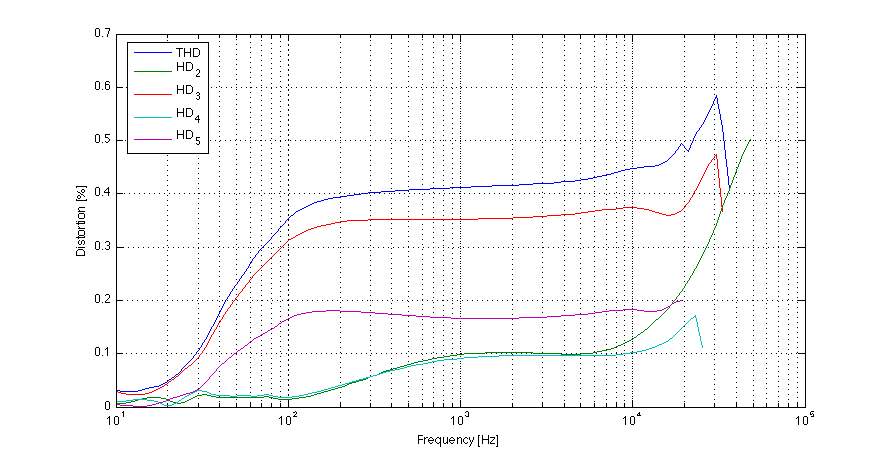
\includegraphics[width=\textwidth]{maalerapporter/effektforstaerker/2V-45mA-uden-modstand-thd.png}
\caption{THD for effektforstærkeren ved 2 V.}
\label{fig:acceff:thd2v}
\end{figure}

Der kan aflæses at THD ved fuld udstyring når et max på ca 0,49\%, ved ca 19 kHz. Dette er under de 0,5\% der er defineret som et krav og er derfor accepteret. 